%! TEX program = xelatex
\documentclass[11pt,a4paper,oneside]{report}

\usepackage{amsmath,amssymb}
\usepackage{parskip}
\usepackage{graphicx}
\usepackage{xcolor}
\usepackage[a4paper,margin=1in]{geometry}
\usepackage{longtable,booktabs,array}

\usepackage{titlesec}
\titleformat{\chapter}[display]
{\sffamily\bfseries\huge}
{\Large \chaptertitlename\ \thechapter}
{2ex}
{\titlerule
    \vspace{1ex}%
    \filright\MakeUppercase}
[\vspace{1ex}%
    \titlerule]
\titleformat{\section}{\normalfont\sffamily\Large\bfseries}{\thesection}{1em}{}
\titleformat{\subsection}{\normalfont\sffamily\large\bfseries}{\thesubsection}{1em}{}
\titleformat{\subsubsection}{\normalfont\sffamily\normalsize\bfseries}{\thesubsubsection}{1em}{}

\usepackage[style=numeric-comp, url=false]{biblatex}
\addbibresource{bibfile.bib}

\usepackage{fontspec}
\setmainfont{TeX Gyre Termes}
\setsansfont{TeX Gyre Termes}

\usepackage{xeCJK}
\setCJKmainfont{Songti SC}
\setCJKsansfont{Songti SC}
\setCJKmonofont{Songti SC}

\newcommand{\instructions}[1]{{\color{orange}\itshape #1}}
\renewcommand{\instructions}[1]{} % Uncomment this to hide the instructions.

\usepackage{upquote}
\usepackage[allcolors=blue,colorlinks=true]{hyperref}
\usepackage{xurl}
\usepackage{microtype}
\usepackage{bookmark}
\usepackage{calc}
\usepackage{etoolbox}

\urlstyle{same}

\usepackage{pifont}  % for the checkmark/crossmark
\usepackage{graphicx}

\usepackage{algorithmic}
\usepackage[ruled]{algorithm2e}

\usepackage{xspace}
\newcommand{\fedcampus}{\textsc{FedCampus}\xspace}
\newcommand{\fedkit}{\textsc{FedKit}\xspace}

\begin{document}


% Author name (capitalized in its regular way)
\newcommand{\authorname}{Sichang He}

% Title (cannot exceed three lines)
\newcommand{\thetitle}{Integrating Federated Learning for \fedcampus,
    A Privacy-Preserving Data Platform for Smart Campus
}

% Date of submission with normal capitalization. Use the format January 29, 2022.
\newcommand{\submissiondate}{March 7, 2024}

% Mentor: First Name Last Name (normal capitalization)
\newcommand{\mentor}{Bing Luo}

% Academic Unit (no abbreviations)
\newcommand{\academicunit}{Division of Natural and Applied Sciences}

%%%%%%%%%%%%%%%%%%%%%%%%%%%%%%%%%%%%%%%%%%%%%%%%%%%%%%%%%%%%%%%%%%%%%%%%%%%%%%%%

%% DO NOT CHANGE DIRECTLY THE CONTENTS OF THE TITLE PAGE.
%% TO CUSTOMIZE THE TITLE PAGE CHANGE THE DEFINITIONS OF THE COMMANDS
%% \authorname, \thetitle, \submissiondate, \mentor, \academicunit

\begin{titlepage}

    \vspace*{\bigskipamount}

    \begin{center}
        {\sffamily\LARGE\bfseries\MakeUppercase\thetitle\par}

        \bigskip

        by

        \bigskip

        {\Large \authorname}

        \bigskip

        Signature Work Product, in partial fulfillment of the \\
        Duke Kunshan University Undergraduate Degree Program

        \bigskip

        \emph{\submissiondate}

        \bigskip

        Signature Work Program \\
        Duke Kunshan University

    \end{center}

    \vfill

    \textbf{\textsf{APPROVALS}}

    \bigskip\bigskip\bigskip
    \hrule

    Mentor: \mentor, \academicunit

    \bigskip\bigskip\bigskip
    \hrule

    Marcia B. France, Dean of Undergraduate Studies

\end{titlepage}

%%%%%%%%%%%%%%%%%%%%%%%%%%%%%%%%%%%%%%%%%%%%%%%%%%%%%%%%%%%%%%%%%%%%%%%%%%%%%%%%

% Front matter
\clearpage
\pagenumbering{roman}

%%%%%%%%%%%%%%%%%%%%%%%%%%%%%%%%%%%%%%%%%%%%%%%%%%%%%%%%%%%%%%%%%%%%%%%%%%%%%%%%

\setcounter{tocdepth}{0} % Only top-level units (chapters) should appear in the TOC
\tableofcontents

%%%%%%%%%%%%%%%%%%%%%%%%%%%%%%%%%%%%%%%%%%%%%%%%%%%%%%%%%%%%%%%%%%%%%%%%%%%%%%%%

\chapter*{Abstract}
\addcontentsline{toc}{chapter}{Abstract}

% Abstract in English

\instructions{Abstract (English): 150 -- 200 words. An abstract is a brief
    statement of the problem or the purpose of the research. It should indicate
    the theoretical work or experimental plan used, summarize principal findings
    of the research, and point out major conclusions. Appropriate safety
    information should be included when applicable. This should be the section
    you write last to be sure that it accurately reflects the content of the
    document.}

\fedcampus aims to build a data platform for university campus that derives
insights from data on campus while preserving participants' privacy.
As a first step towards this goal,
we developed solutions for accessing personal health data on participants'
smartphones and conducting cross-platform federated learning.
Federated learning is a privacy-preserving machine learning technique that
enables training machine learning models across multiple edge devices without
centralizing the raw data,
but it faces major challenges in cross-platform federated learning on
smartphones including cross-platform support, dependency on application update,
and interdisciplinary collaboration. We developed \fedkit,
software development kits that address these challenges through a machine
learning model pipeline and machine learning operations support.
Our experiments were carried out both on lab-based setting,
and on The \fedcampus Application,
which was deployed among tens of participants including students,
staff and faculty on Duke Kunshan University campus.
The results demonstrated the effectiveness of \fedkit and the feasibility of
\fedcampus' overall approach.

\vspace{4\bigskipamount}

% Abstract in Chinese

\instructions{摘要(中文):150 - 200
    字。摘要是对问题或研究目的的简要说明。说明所使用的理论工作或实验计划,总结研究的主要发现,
    并指出主要结论。适用时应包括适当的安全信息。这应该是您最后编写的部分,
    以确保它准确反映文档的内容。}


%%%%%%%%%%%%%%%%%%%%%%%%%%%%%%%%%%%%%%%%%%%%%%%%%%%%%%%%%%%%%%%%%%%%%%%%%%%%%%%%

\chapter*{Acknowledgements}
\label{acknowledgements}
\addcontentsline{toc}{chapter}{Acknowledgements}

\instructions{Individuals and organizations who helped with the research project
    and provided financing are thanked in a paragraph of the thesis. Do not
    include individual titles in the acknowledgments. However, it is
    appropriate to state grant numbers and sponsors. Examples would like
    SELF, SRS, SW Grants, etc.}

This project is supported by Duke Kunshan University Undergraduate Office via
the Summer Research Scholars Program. Thanks to all \fedcampus team members and
alumni; your hard work made this project possible.
Special thanks to our chief developer Beilong Tang and our shepherd Jiaqi Shao.

\newpage

%%%%%%%%%%%%%%%%%%%%%%%%%%%%%%%%%%%%%%%%%%%%%%%%%%%%%%%%%%%%%%%%%%%%%%%%%%%%%%%%

% Add captions to your figures for them to appear in the List of Figures.
% Alternatively, comment out the next two lines if there are no tables 
% in your document.
\addcontentsline{toc}{chapter}{List of Figures}
\setcounter{tocdepth}{1}
\listoffigures\newpage

%%%%%%%%%%%%%%%%%%%%%%%%%%%%%%%%%%%%%%%%%%%%%%%%%%%%%%%%%%%%%%%%%%%%%%%%%%%%%%%%

% Add captions to your tables for them to appear in the List of Tables.
% Alternatively, comment out the next two lines if there are no tables 
% in your document.
\addcontentsline{toc}{chapter}{List of Tables}
\setcounter{tocdepth}{1}
\listoftables\newpage

%%%%%%%%%%%%%%%%%%%%%%%%%%%%%%%%%%%%%%%%%%%%%%%%%%%%%%%%%%%%%%%%%%%%%%%%%%%%%%%%

% Main matter
\clearpage
\pagenumbering{arabic}

%%%%%%%%%%%%%%%%%%%%%%%%%%%%%%%%%%%%%%%%%%%%%%%%%%%%%%%%%%%%%%%%%%%%%%%%%%%%%%%%

\chapter{Introduction}
\label{introduction}

\instructions{This section includes a clear statement of the problem and the
    reasons for studying it.~Provide a detailed yet concise background
    discussion of the problem and the significance, scope, and limits of the
    work. Outline what has been done previously by citing truly pertinent
    literature but do not include a general survey of semi-relevant
    literature.~ State how your work differs from earlier work in the field
    and demonstrate the continuity from the previous work to your own.}

\section{Federated Learning}

\section{Federated Analytics}

\section{Healthcare Data Analytics}


%%%%%%%%%%%%%%%%%%%%%%%%%%%%%%%%%%%%%%%%%%%%%%%%%%%%%%%%%%%%%%%%%%%%%%%%%%%%%%%%

\chapter{Methods}
\label{methods}

\instructions{This section is obviously discipline specific so use the
    nomenclature that is common for your discipline. However, this section
    should provide sufficient detail about the materials and the methods
    used so that other experienced workers can repeat the experiment and
    obtain comparable results. Cite the appropriate literature when using a
    standard method or protocol and give only the details needed. Identify
    the materials used in the research. For example, computer systems used,
    mathematical theorems exploited, etc.; give information on the purity of
    all chemicals and reagents employed in the research; include the
    chemical/biological names of all compounds and chemical formulas of
    substances that are new or uncommon. Use standard systematic
    nomenclature to unambiguously define well-established compounds,
    processes, equipment, etc.}

\section{General Federated Learning Procedure}

\begin{algorithm}
    \caption{General Federated Learning Procedure}
    \label{algo:general-procedure}
\ForEach{Training iteration}{
Distribute the global model to all clients\;
\ForEach{Client}{
    Train the local model using local training data\;
    Send the trained local model back to the central server\;
}
The central server aggregates all local models into a new global model\;
}
\end{algorithm}

The general procedure of federated learning on mobile devices involves a
distributed system with two parties: the clients and the central server.
The process unfolds through training iterations, with four phases per iteration,
as illustrated in Algorithm~\ref{algo:general-procedure}. In each iteration,
the central server distributes the global model to clients,
who then train the global model locally using their individual data.
Trained local models are sent back to the central server,
and these models are aggregated to generate an updated global model.
This process repeats for successive iterations.
In the context of federated learning on mobile devices,
clients are typically mobile applications on Android or iOS devices,
and the central server is a remote server on the Internet,
as depicted in Fig.~\ref{fig:general-fl}.

\begin{figure}\begin{center}
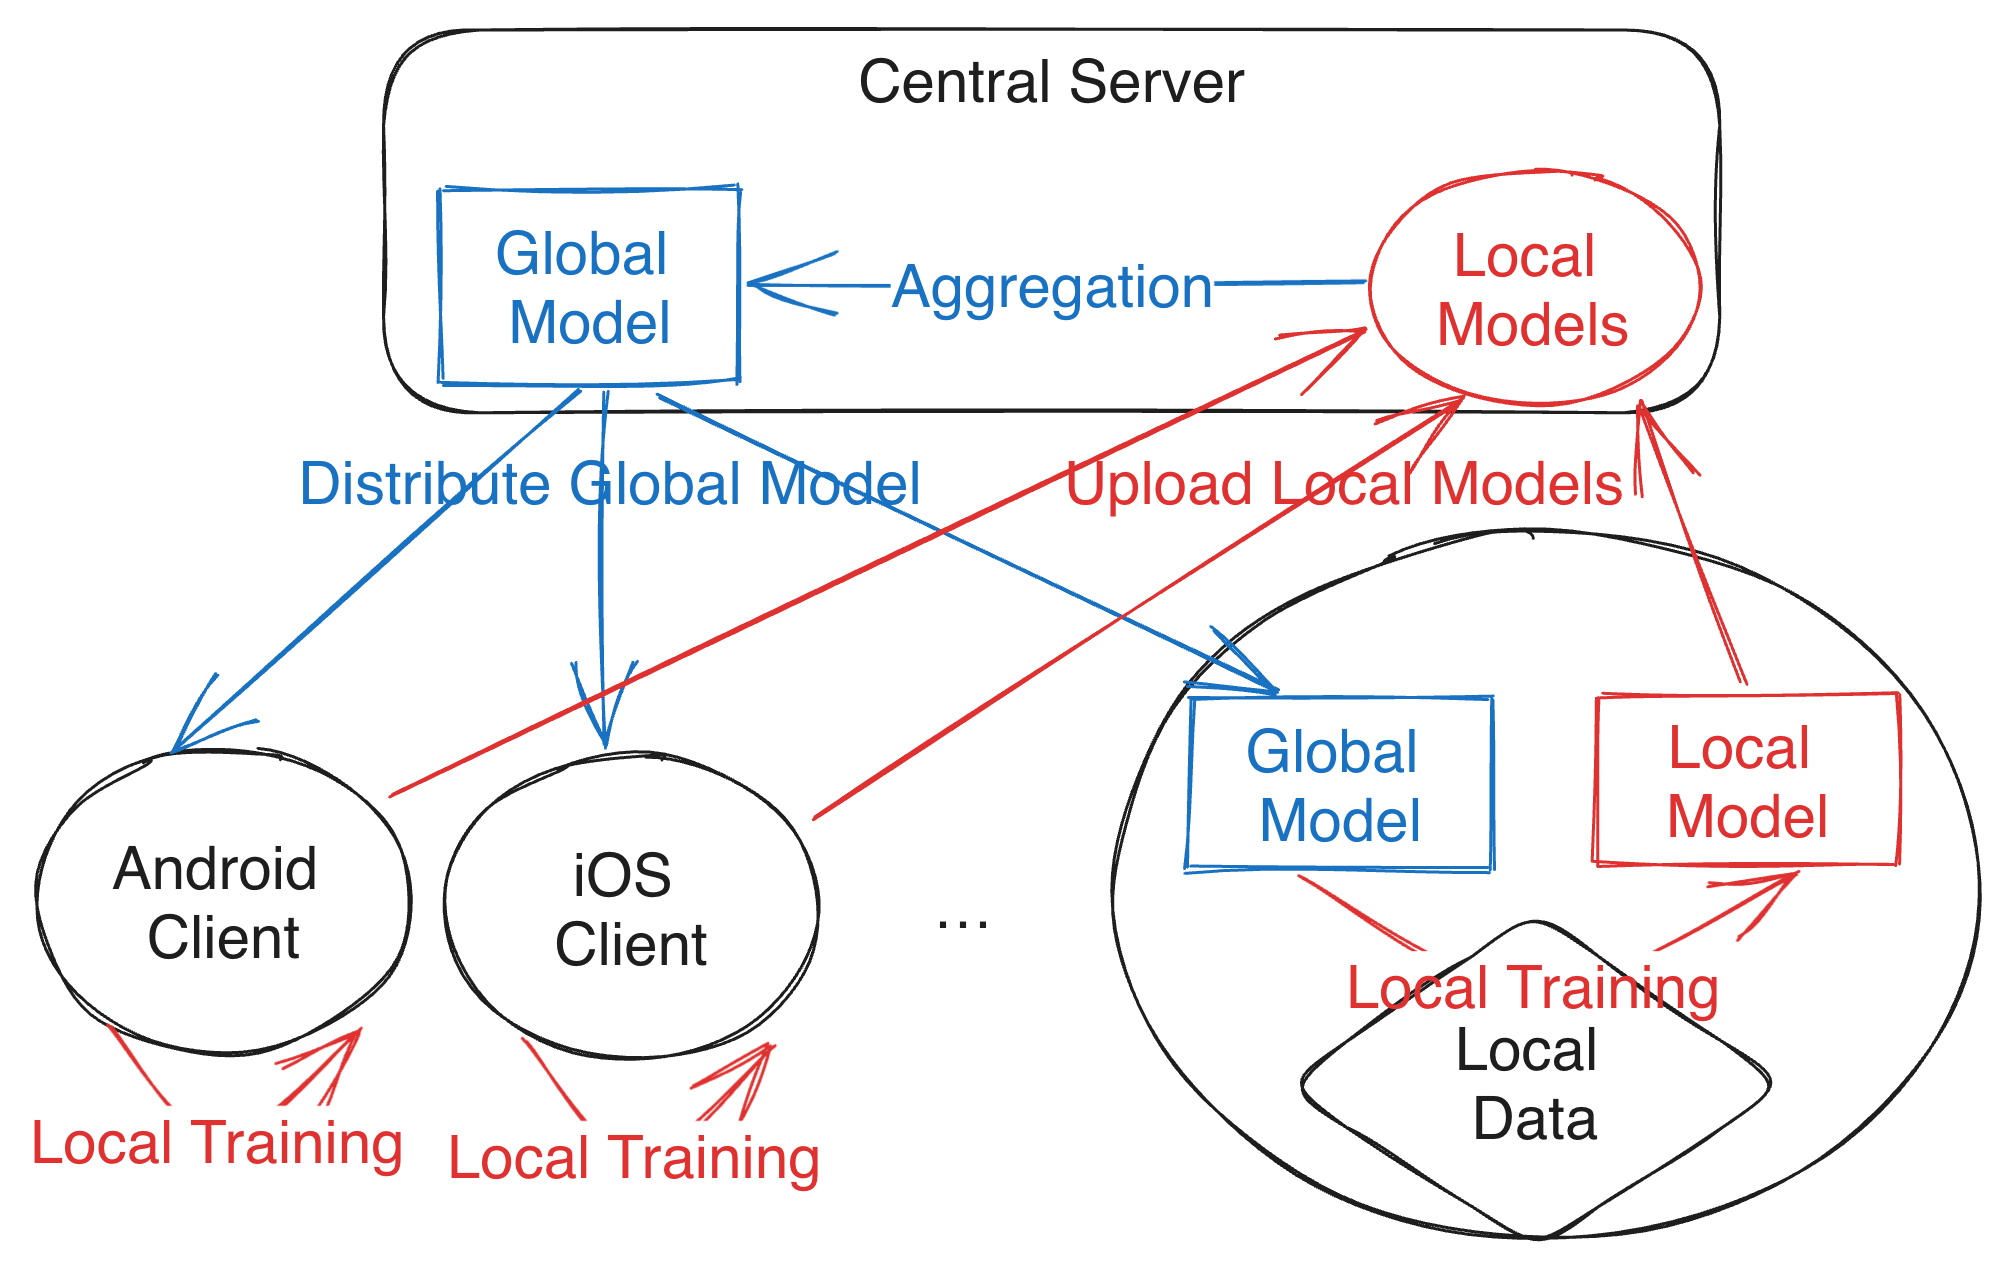
\includegraphics[width=0.7\textwidth]{general_fl.png}
    \caption{General Federated Learning Procedure on Smartphones.}
    \label{fig:general-fl}
\end{center}\end{figure}

The specific implementations of federated learning on mobile devices may vary,
but they share a common foundation. The FedAvg algorithm,
presented with federated learning itself~\cite{mcmahan2017communication},
stands as the most typical federated learning algorithm. In FedAvg,
a fixed number of $C$ out of $K$ clients are selected for local training in each
iteration.
The local training aims to minimize the loss $L$ of the model for each client's
local data partition $P_k (k \in \{1, 2, \dots, K\})$:
\begin{equation}
\min_{w_k} L(P_k;w_k),
\end{equation}
starting from the parameters $w^{(t)}$ of the latest global model from the
server, and scheduled for a fixed number of $E$ epochs.
To optimize the global model for the entire training dataset $\bigcup_k P_k$,
FedAvg aims to minimize the weighted average of local losses
\begin{equation}
\min_{w} \frac{\sum_k |P_k|L(P_k;w)}{\sum_k |P_k|},
\text{ where }|P_k|\text{ is the size of }P_k,
\end{equation}
by computing the weighted average of local models' weights
\begin{equation}
w^{(t+1)}=\sum_k \frac{|P_k|}{\sum_k |P_k|}w_k^{(t+1)}
\end{equation}
to update the global model.
This iteration is repeated until model convergence or experiment termination.
FedAvg has proven effective and practical in various experimental scenarios,
benchmarked against earlier algorithms in data center
settings~\cite{bonawitz2019towards}.

\section{Machine Learning Operations}

% TODO: Improve this and cite.
Machine learning operations (MLOps) is a set of practices similar to
development operations (DevOps).
In development operations,
the software development process and the deployment process are integrated,
so that new software changes made by the development team can be
automatically deployed into production.
Similarly, in machine learning operations,
changes in the machine learning algorithms can be automatically deployed into
production.
Machine learning operations is desirable when the development velocity on
the machine learning algorithms is high,
and feedbacks from the production environment are important to improve
the machine learning algorithms.


%%%%%%%%%%%%%%%%%%%%%%%%%%%%%%%%%%%%%%%%%%%%%%%%%%%%%%%%%%%%%%%%%%%%%%%%%%%%%%%%

\chapter{Design}
\label{design}

\section{Data Access}

\paragraph{Ground Truth}
To preserve user privacy,
the bottom line is that the raw data must not be collected.

The initial phase of FedCampus operates on participants' health data recorded by
the Huawei Watch Fit 2.
100 smartwatches of this model are purchased to be lent to the participants.

In order to conduct research on the data,
our algorithm needs to access the data from the smartwatch.

In the natural life cycle of the collected health data,
the data are first synchronized from the participants' smartwatches to
the Huawei HealthKit on the their smartphone through Bluetooth.
This is important in two ways:
first, we do not need to develop any software to run on the smartwatches,
only the smartphones; second,
we require the participants to regularly conduct this synchronization process
themselves, which counts into management complexity.

We deploy different strategies to access the data from the Huawei HealthKit on
Android and iOS.
On Android, Huawei provides the Huawei HealthKit API to access the data.
On iOS, Apple restricts third-party access to private data,
and unifies such access to Apple HealthKit,
so we have to first synchronize the data from the Huawei HealthKit to
the Apple HealthKit, then access the data via Apple HealthKit.

\section{The \fedcampus Application}

The major challenge of the \fedcampus Application is to
support both Android and iOS devices.
This is necessary because our participants at Duke Kunshan University are
a mix of Android and iOS users,
and we want to allow as many of them to participate as possible.
However, Android and iOS applications are incompatible,
and developing separate applications for these two platforms would be
a laborious task because
it would mean we have to maintain two separate codebases and
duplicate any changes.

To support mobile development on both Android and iOS,
we leverage the Flutter application framework.
Instead of developing two separate applications for Android and iOS,
by using Flutter,
only a single codebase is needed to for both the Android and iOS versions of
the application.
Therefore, we implement as much of the \fedcampus Application on Flutter as
possible to maximize our code reuse and minimize our development effort.


%%%%%%%%%%%%%%%%%%%%%%%%%%%%%%%%%%%%%%%%%%%%%%%%%%%%%%%%%%%%%%%%%%%%%%%%%%%%%%%%

\chapter{Implementation}
\label{implementation}

\section{Accessing the Data}

On Android, we use the Huawei Health Kit API Java package to request
Huawei Health Kit for the data.
This API allows access to all the collected raw health data points.
We call the API from using Kotlin,
a programming language compatible with Java,
and aggregate the data into a daily summary.
% TODO: What are the data types.
We used Kotlin to integrate with Huawei Health Kit API because
we found it to be more concise and maintainable than Java while
having complete interoperability.
A special pop-up authentication page is also implemented to request the user for
permissions to access their health data, as required by Huawei.

On iOS, we indirectly access Apple HealthKit through Flutter's
Health~\cite{flutterhealth} package.
The Health package provides a unified interface to access health data,
and notifies iOS to request permissions from the user to access the health data.
Since the Health package can also request health data from Google Fit on
Android, we provide an optional feature to use health data from Google Fit to
experimentally accommodate participants who use Android smartphones and
do not use Huawei smartwatches.

In our internal testing, we noticed that accessing the data could be slow,
especially when requesting data using the Huawei Health Kit API.
To mitigate this issue, we implemented a local cache database.
Before we request data from either of the health kits,
we first check the cache database for the data.
If the data is not in the cache database,
we request the data from the health kit and update the cache database.
% TODO: Not implemented yet.
We also implemented a background task to periodically update the cache database,
and the users can also force an update by refreshing the health page in
the application.

\section{The \fedcampus Application}

Most of the \fedcampus Application is implemented in Dart using
the Flutter application framework, with a few exceptions.
The data access on Android and the federated learning on-device training part
calls into platform-specific native code under Flutter's mechanism.

We leverage Flutter's strong support for
building attractive user interface to fulfill the need to
create a user-friendly application.
Additional, HTTP request libraries and JSON libraries in Dart are used to
communicate with the backend,
and an SQL library is used to manage the cache database.

\section{\fedkit}

Overall, \fedkit powers a federated learning system that
consists of a single backend server and a set of mobile application clients.
The clients train their local models on-device with their local data,
and exchange machine learning models and parameters with the backend server to
conduct federated learning.

\begin{table}\begin{center}
    \begin{tabular}{llll}
Library&Functionality&Language&Framework\\\hline
Backend Server&Training Orchestration \& Telemetry&Python&Django\\
Flutter Flower Client&Backend \& FL Server Communication&Dart&Flutter\\
TensorFlow Lite Trainer&Training on Android&Kotlin&TensorFlow Lite\\
TensorFlow Lite Converter&TensorFlow Models Conversion&Python&TensorFlow\\
Core ML Trainer&Training on iOS&Swift&Core ML
    \end{tabular}
    \caption{Major Libraries in the \fedkit Software Development Kit.}
\label{table:libs}
\end{center}\end{table}

\fedkit implements 5 libraries, as listed in Table~\ref{table:libs},
to manage client-server communication and simplify on-device machine learning
training.

The backend server orchestrates the federated learning process and persists
relevant information in a database through the object-relational mapping the
Django web framework provides. We used SQLite for the database during testing,
and replaced it with PostgreSQL in the deployment. In our deployment,
each model is first uploaded to the backend server,
where model files are stored using the file system and model information is
stored in the database.
Model information is used to determine which clients a model support.
It include whether the model supports TensorFlow Lite or Core ML training,
and a fixed data type that specifies the shape of training input tensors and
labels.
Client applications are bundled with a specific implementation to obtain a
certain data type,
which they use to request the backend server for compatible models.

To reduce the development and maintenance cost operating on both Android and
iOS,
we adopted the Flutter framework to implement the client in our applications to
communicate with the Flower federated learning servers spawned by the backend
server. Since the Flower server leverages gRPC to connect to the clients,
we used the Dart gRPC package to implement the client according to Flower's
protocols.
% TODO: Cite Anthony's Flower Flutter client.
While we intend to record additional telemetry information during training,
we do not want to modify the internals of the Flower servers. Therefore,
we also rely on the Flutter clients to send telemetry information to the backend
server via our representational state transfer application programming
interfaces.
Besides communicating with the backend server and the Flower server,
the Flutter clients also manage the on-device training process by calling into
the platform specific trainers. % TODO: Cite Flutter platform channels.

The TensorFlow Lite Converter is a thin wrapper around TensorFlow to convert
TensorFlow models to the TensorFlow Lite models format we defined in
Section~\ref{sec:pipeline}.
To convert TensorFlow models to Core ML models,
we use the CoreMLTools Python package developed by Apple. After the conversion,
we extract the information about the model layers. For TensorFlow Lite models,
we extract a list of all layers' parameter sizes; for Core ML models,
we extract the layer names, whether they are weights or biases,
and whether they are updatable.
This information is used when aggregating the models and updating the model
parameters on the client, as also discussed in Section~\ref{sec:pipeline}.

While the TensorFlow Lite Trainer directly call the functions defined in the
TensorFlow Lite models, known as ``signatures'',
to complete all federated learning tasks,
the Core ML Trainer additionally uses the Swift ProtoBuf package to inspect and
modify the Core ML model files directly.
% TODO: Cite the Flower Core ML example.
Before training a Core ML model,
we use ProtoBuf to extract all of the model's layers.
To update the model during federated learning,
we use ProtoBuf to manipulate the layer weights and biases in the model file,
and recompile it into a new model,
therefore working around Core ML's artificial prohibition on updating the model
file.


%%%%%%%%%%%%%%%%%%%%%%%%%%%%%%%%%%%%%%%%%%%%%%%%%%%%%%%%%%%%%%%%%%%%%%%%%%%%%%%%

\chapter{Results}
\label{results}

\instructions{Summarize the data collected in this section, and their
    statistical treatment. Include only relevant data, but give sufficient
    detail to justify the conclusions. It is appropriate in this section to
    use equations, figures, and tables to display your data. Extensive, but
    relevant data, should be reserved for an appendix where it is identified
    as supporting information.}

\instructions{The table or figure must follow as closely as possible after the
    paragraph in which it is referenced. Titles/captions should be kept
    brief.}

\instructions{
    \section{Examples}

    Here is some inline math, $x^2 > 1$, and some display math
    \begin{equation}
        \int_0^1 x^2 \, dx
    \end{equation}
    And this is how to cite an article \cite{Zhang2021} or a book \cite{Axler2020}.

    \begin{table}[htbp]
        \centering
        \begin{tabular}{@{}llll@{}}
            \toprule
            \emph{Replace} & \emph{With} & \emph{Your} & \emph{Table} \\
            \midrule
                           &             &             &              \\
                           &             &             &              \\
            \bottomrule
        \end{tabular}
        \caption{Parameters for the optimization of the principal component analysis for
            olive oil adulteration.}
        \label{tbl:2}
    \end{table}


    \begin{figure}[htbp]
        \centering
        \includegraphics[height=4cm]{btc.jpg}
        \caption{The notorious BTC (Brandon The Cat).}
        \label{fig:1}
    \end{figure}
}

\section{The \fedcampus Application}

\begin{figure}\begin{center}
        \label{fig:fedcampus-app}
        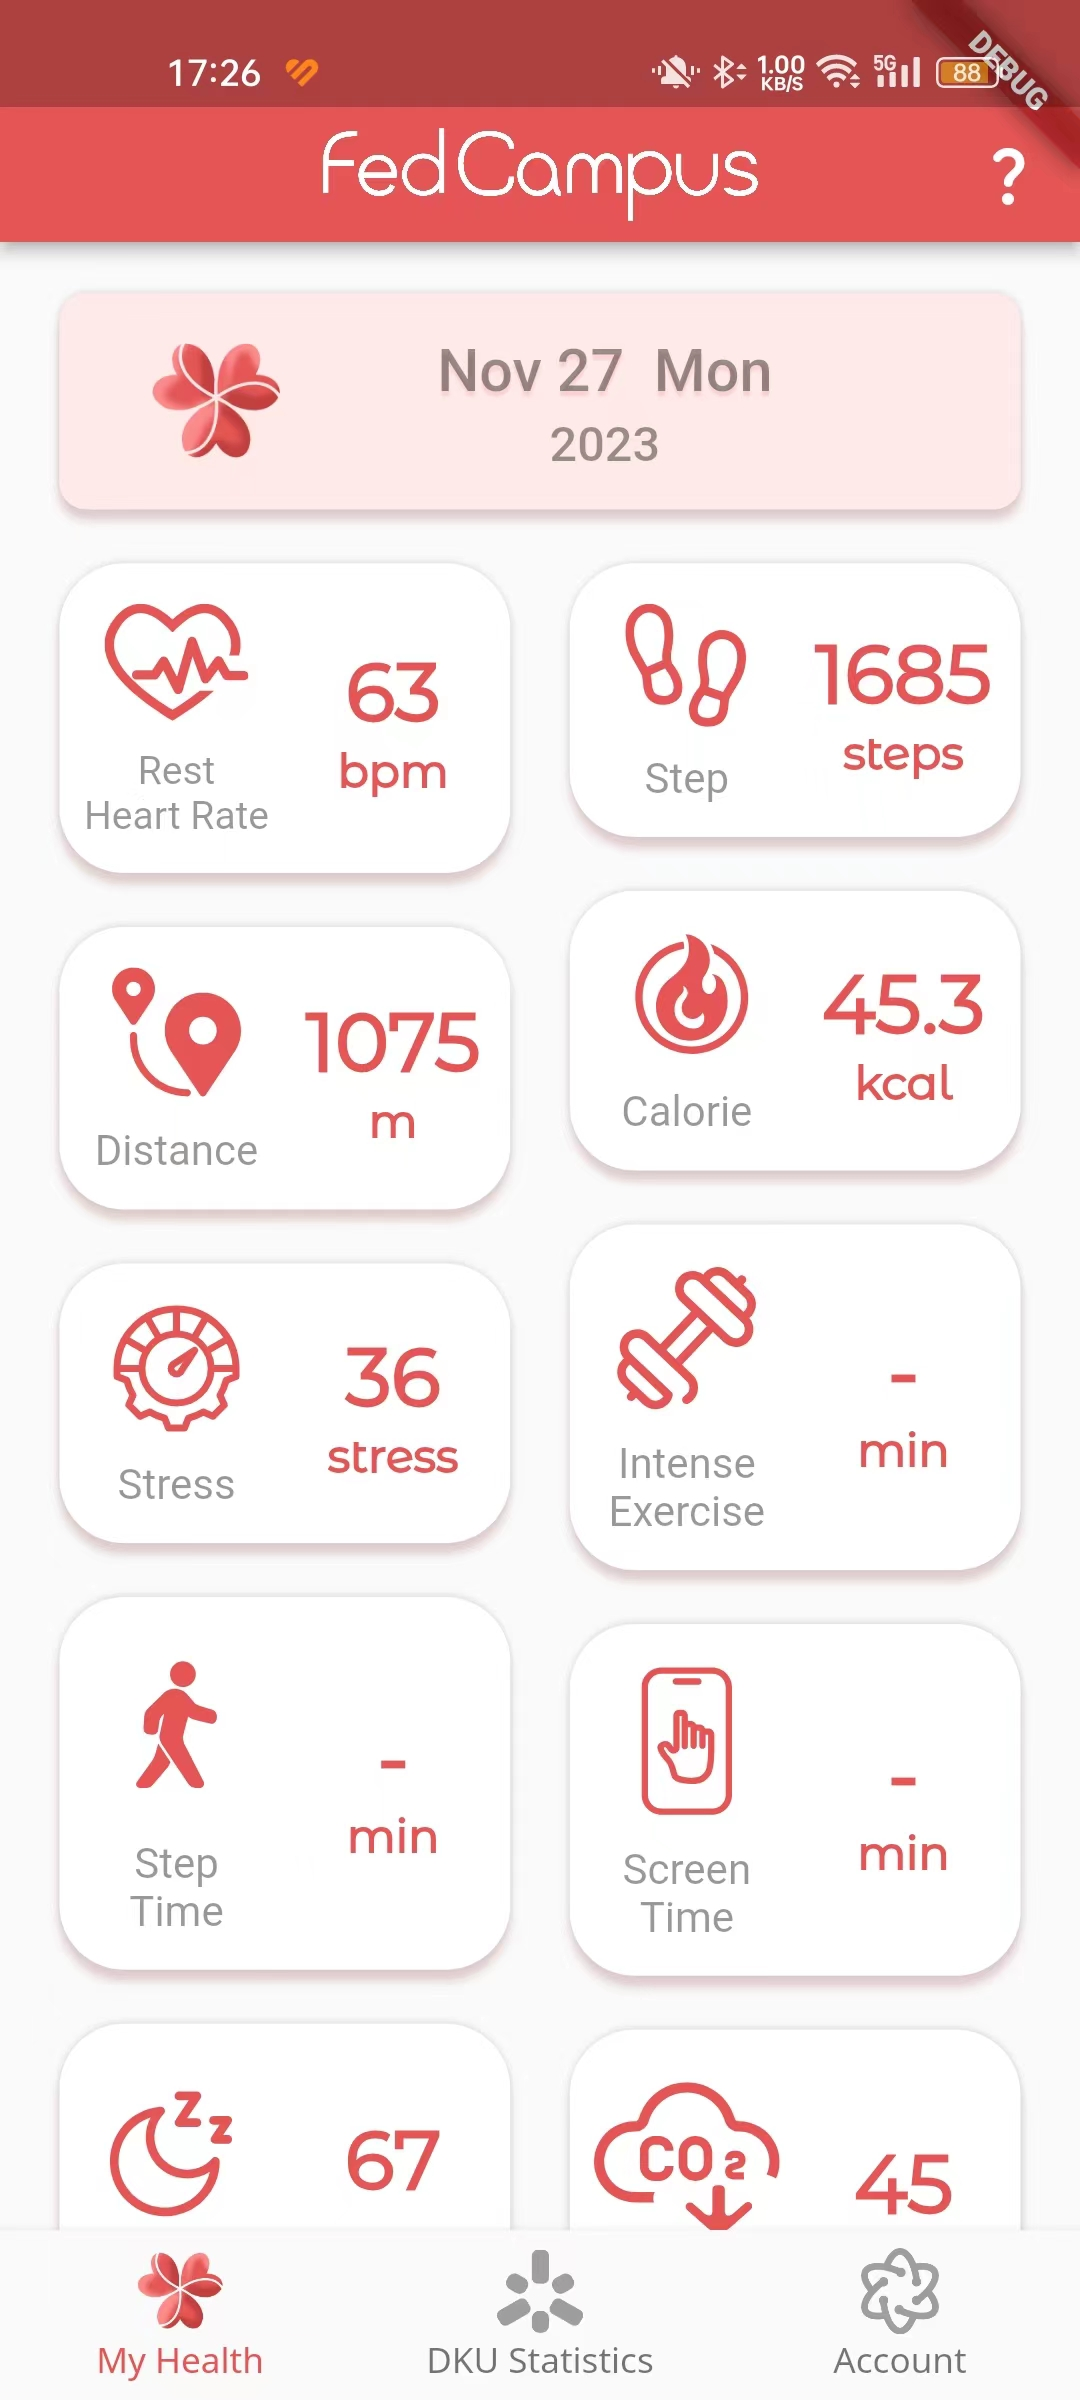
\includegraphics[width=0.3\linewidth]{fedcampus_screenshot1.jpeg}
        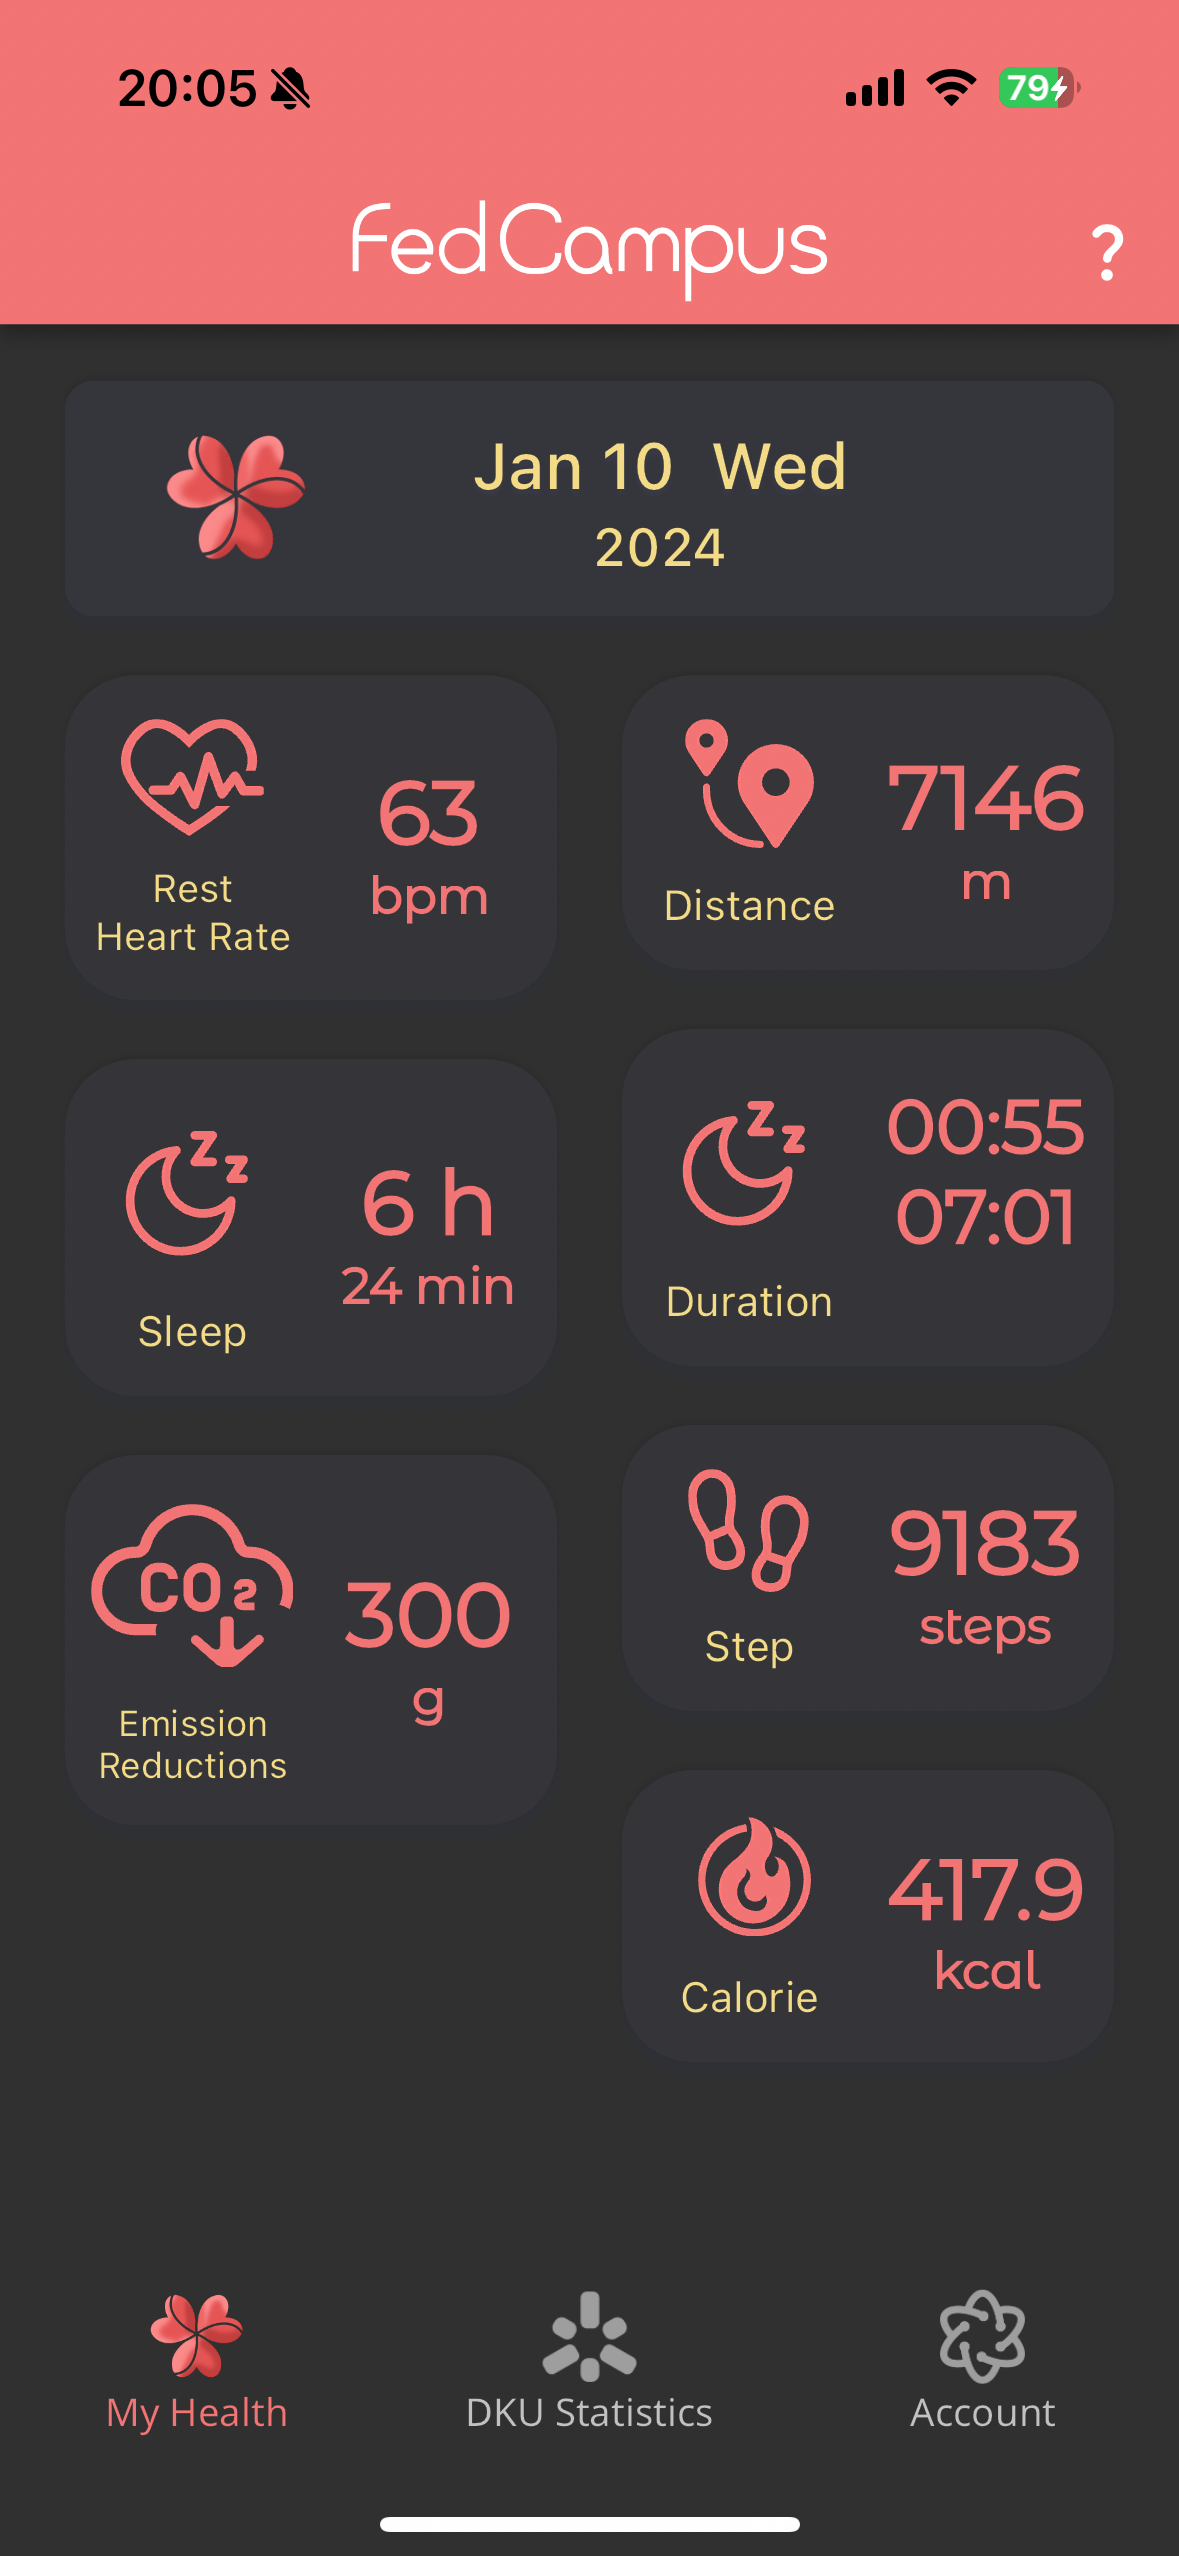
\includegraphics[width=0.31\linewidth]{fedcampus_screenshot3.png}
        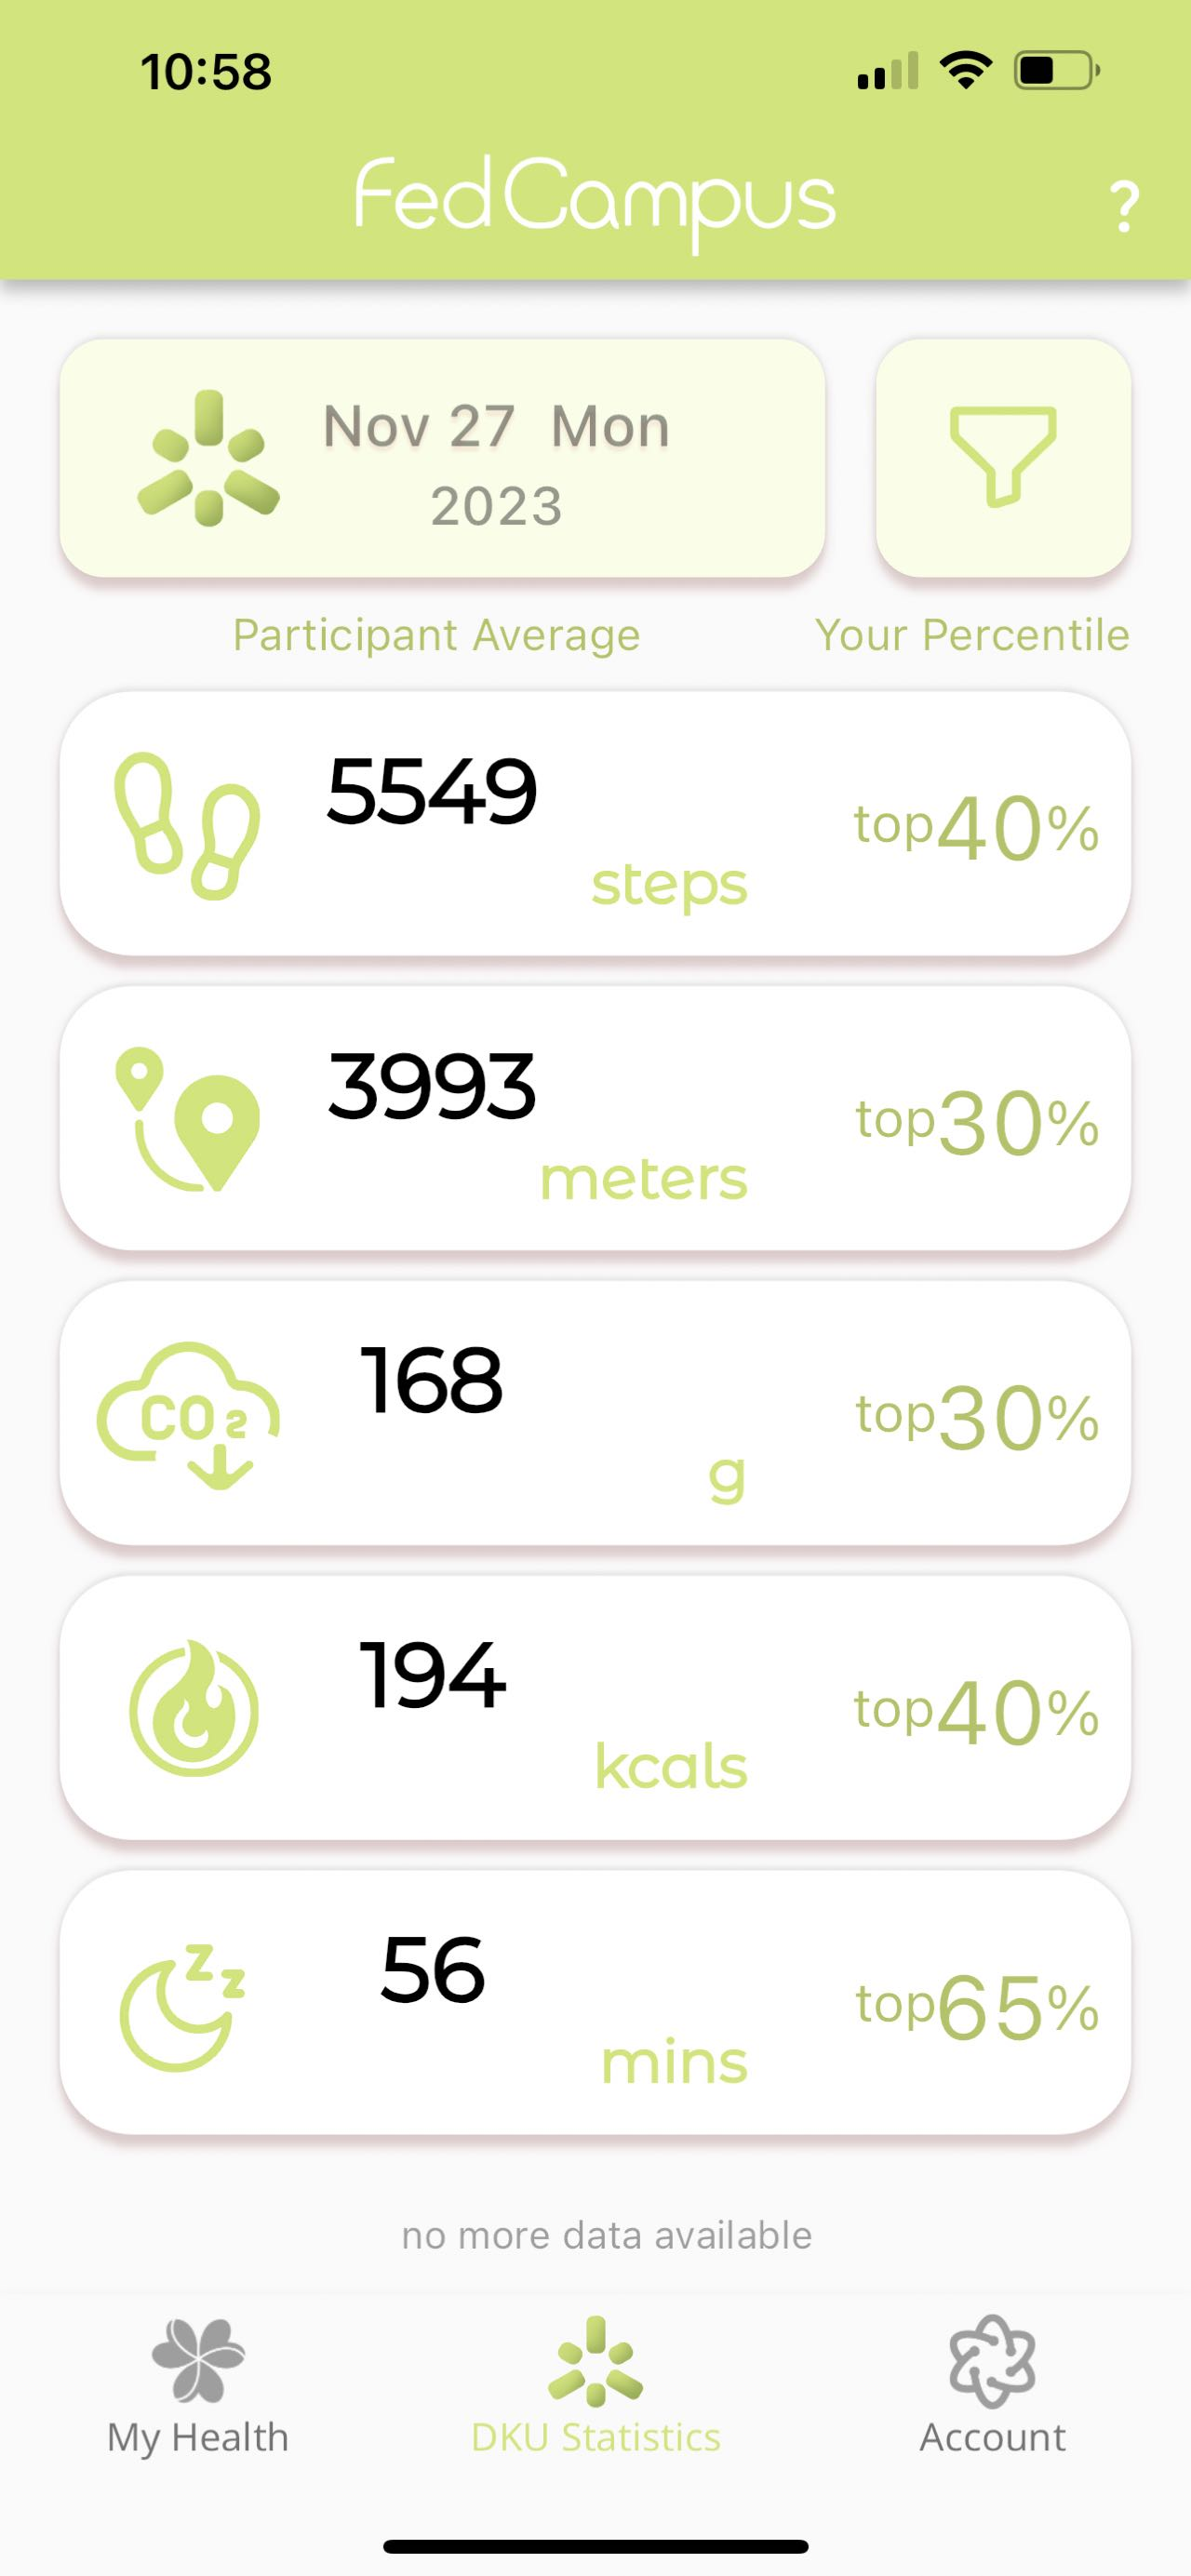
\includegraphics[width=0.31\linewidth]{fedcampus_screenshot2.jpeg}
        \caption{Screenshots of The \fedcampus Application.
            On The left, The User's Personal Health Page on Android;
            On The Middle, The User's Personal Health Page on iOS in Dark Mode;
            On The Right,
            The Group Mean And The User's Approximate Percentile Within The
            Group From Federated Analytics.
        }
    \end{center}\end{figure}

We launched the \fedcampus Application among Duke Kunshan University students,
faculty, and staff in November 2023.
At launch,
the \fedcampus Application displays the users' personal health data accessed,
as well as some statistics derived from federated analytics (see \ref{app:fa}),
as shown in Figure~\ref{fig:fedcampus-app}.
We offered the opportunity to participate in \fedcampus either by lending them
Huawei smartwatches or by using their own Huawei smartwatches.
The \fedcampus Application currently has 93 registered users and approximately
half of them are daily active users.

\subsection{\fedcampus Participant Requirements}

Our involved data access setup results in involved participant requirements.

In practice, accessing the data via the Huawei Health Kit on Android only works
well for participants using Huawei smartphones.
On Huawei smartphones,
the operating system automatically periodically synchronizes health data from
the connected Huawei smartwatch to the Huawei Health Kit.
Therefore, when these participants launch our FedCampus Application,
the app can immediately access the latest data from the Huawei Health Kit.

However, on non-Huawei Android smartphones,
the synchronization from the smartwatches only happens when
the Huawei Health app is on the foreground,
unless participants install Huawei Management System Core (HMS Core),
a background service app.
Alpha testers reported that the HMS Core is battery-consuming,
and is sometimes shut down by the operating system on smartphones made by
Xiaomi and other companies.
Additionally, Huawei apps are not available on the Google Play Store,
so some participants also have to install the Huawei AppGallery Application.
This makes an undesirable experience where the participants are required to
install four different apps.
Despite the inconveniences, once the participants have installed the apps,
they do not need to conduct this process again.

On iOS, participants can download the Huawei Health app from the App Store,
but it does not synchronize data from the Huawei smartwatch in the background.
Participants have to manually open the Huawei Health app,
and leave it in the foreground to synchronize the data both from
the smartwatches to the Huawei Health Kit,
and from the Huawei Health Kit to the Apple HealthKit.
It takes a significant amount of time for Huawei Health Kit to
synchronize the data to Apple HealthKit,
especially for the sleep time data;
as a result, it is common for the FedCampus Application to miss sleep data as
it could not read it from Apple HealthKit.

Due to these practical limitations,
we first prioritized Huawei smartphone users, then iPhone users,
for our initial launch.

\section{\fedkit Demonstrations}

To demonstrate \fedkit's capabilities,
we conducted two demonstrations~\cite{he2024fedkit}.
The first demonstration showcases \fedkit's federated learning model pipeline in
a lab setting,
and the second demonstration showcases \fedkit's integration in the \fedcampus
Application.

\subsection{\fedkit MNIST Demonstration}

\begin{figure}\begin{center}
        \label{fig:lab}
        \includegraphics[width=\linewidth]{mnist_demo_photo.jpeg}
        \caption{A previous \fedkit Demonstration Using A MNIST Model And
            Running on An Android Phone And An iOS Simulator.
        }
    \end{center}\end{figure}

We demonstrate federated learning among
devices running an example Flutter client app,
and a laptop running a \fedkit Backend. Each client has $\frac{1}{10}$ of the
MNIST~\cite{cohen2017emnist} dataset locally,
which is used to participate in the federated learning process.

First, we demonstrate our seamless federated learning model pipeline.
We convert a TensorFlow MNIST multi-layer perceptron model and
conduct federated learning with it across an Android and an iOS device.
A previous demonstration running this model is shown in Figure~\ref{fig:lab}.
Second, to showcase machine learning model operations,
we modify the model and deploy its new version.
As outlined in Table~\ref{tbl:demo-stats},
our telemetry shows that
the iOS device is over 5$\times$ faster in local training despite
having 0.5$\times$ RAM,
illustrating how \fedkit will provide real-world statistics to
enhance federated learning algorithm design.

\begin{table}\begin{center}
        \begin{tabular}{lllll}\toprule
            Device            & System on a Chip  & Acceleration & RAM         & Time   \\\midrule
            Huawei Nova 9 Pro & Snapdragon 778G   & OpenCL       & 8GB LPDDR5  & 3.583s \\
            iPhone 13 mini    & A15 Bionic, 4 GPU & CoreML       & 4GB LPDDR4X & 0.656s \\\bottomrule
        \end{tabular}
        \caption{Configurations of Devices and Average Local Training Time Per Round
            (Two Local Epochs) in A Previous Demo Run.
        }
        \label{tbl:demo-stats}
    \end{center}\end{table}

\subsection{\fedkit Integration in The \fedcampus Application}

\begin{figure}\begin{center}
        \label{fig:integration}
        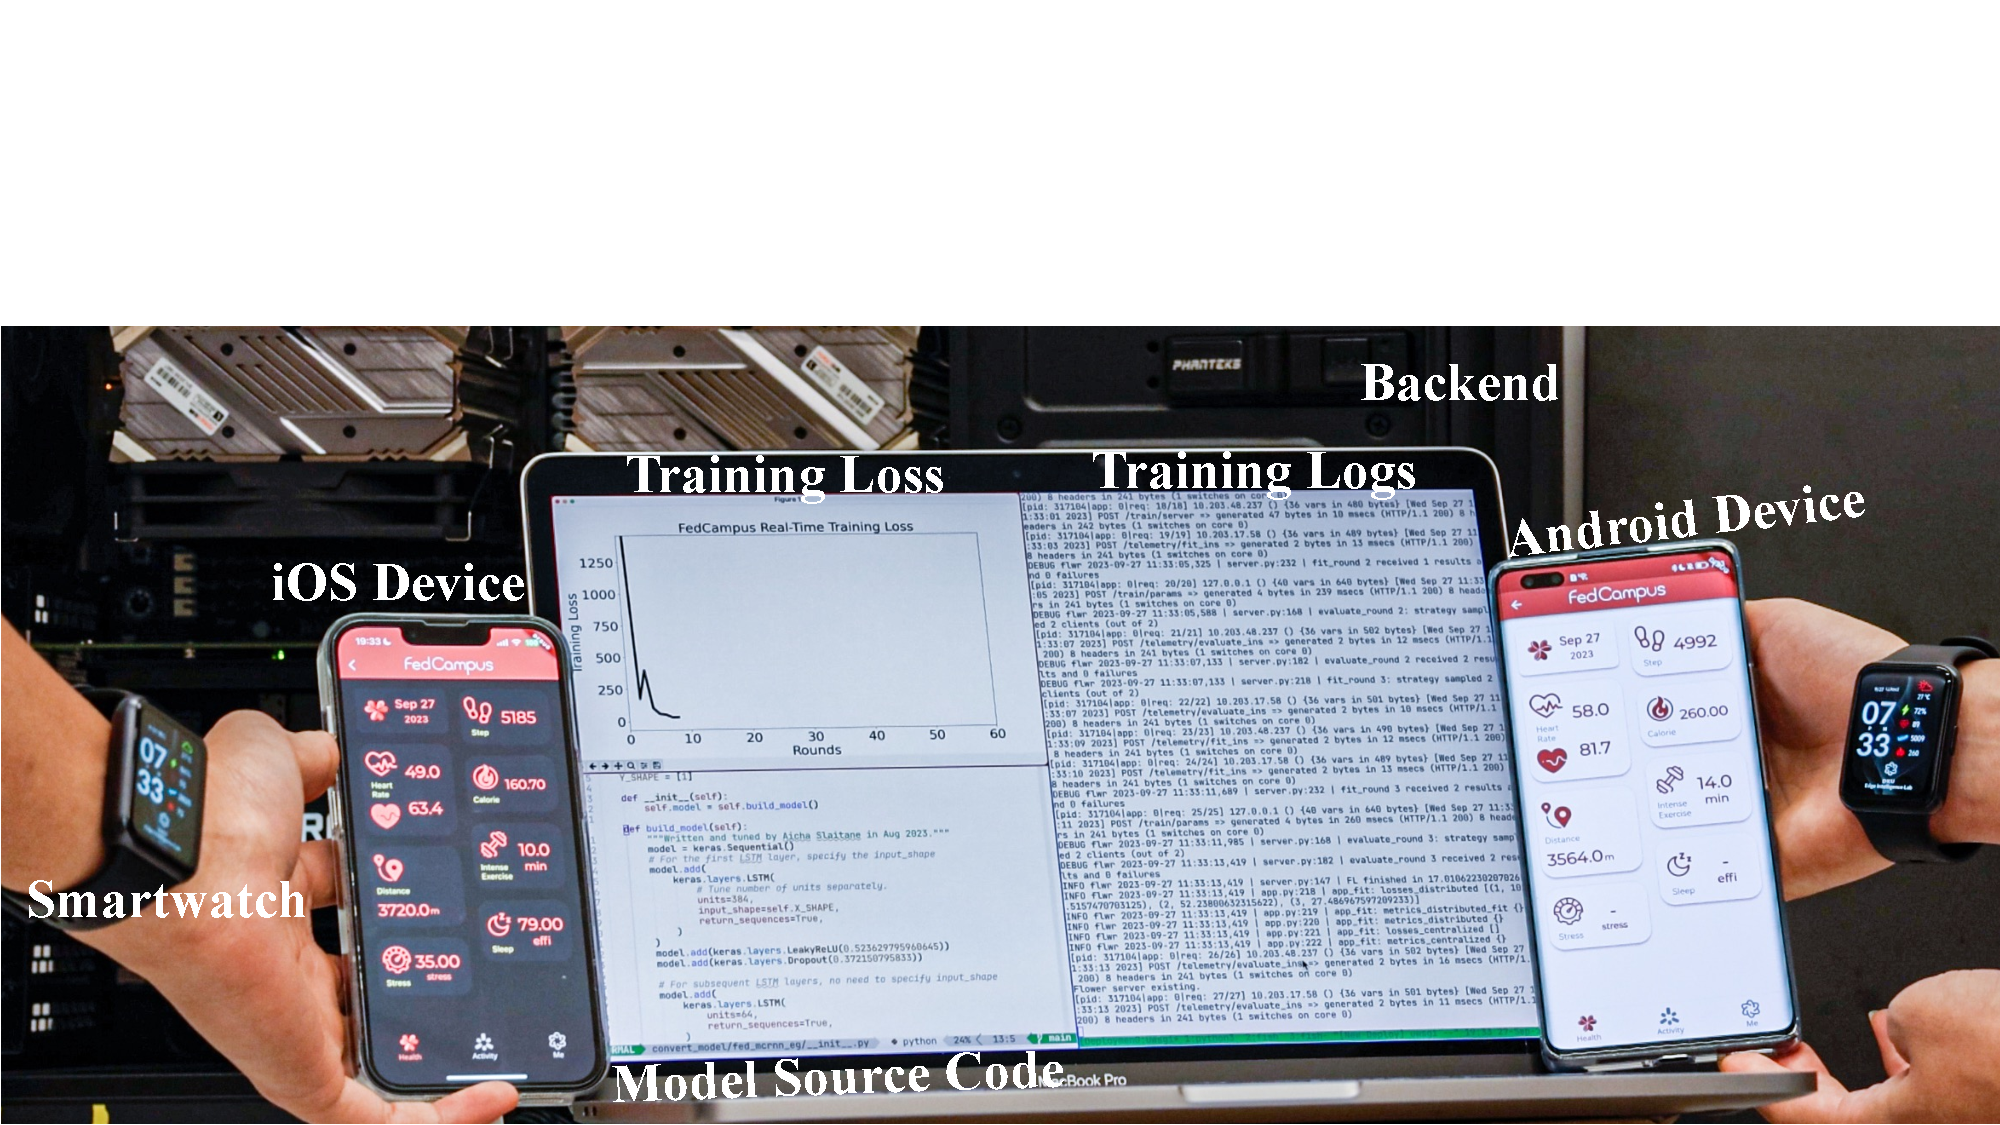
\includegraphics[width=\linewidth]{fedcampus.pdf}
        \caption{Experiment Setup for The \fedkit Integration in The FedCampus
            Application.
        }
    \end{center}\end{figure}

We integrated \fedkit into the \fedcampus Application to
conduct a federated learning experiment using health data on the smartphones,
as displayed in Figure~\ref{fig:integration}.
In our setup,
A backend server is hosted in the physical machine in the background,
while an Android device and an iOS device are running an early version of
the \fedcampus Application.
The laptop is connected to the server via Secure Shell (SSH),
and was displaying the training logs,
along with the training loss and the model's source code.

The \fedcampus Application in this experiment trained a sleep-efficiency
prediction model similar to the model described in~\cite{khoa2022fedmcrnn}
using health data collected from the smartwatches.
Each round of training is instantaneous on both Android because of
the small training dataset,
and both smartphones remained cool with \fedkit's training acceleration.
The models trained on these smartphones are aggregated across Android and iOS,
resulting in a significant reduction in the training loss,
demonstrating \fedkit's effectiveness in real-world scenarios.


%%%%%%%%%%%%%%%%%%%%%%%%%%%%%%%%%%%%%%%%%%%%%%%%%%%%%%%%%%%%%%%%%%%%%%%%%%%%%%%%

\chapter{Discussion}
\label{discussion}

\instructions{The discussion section is where you interpret and compare the
    results. The objective is to point out the features and limitations of
    the work. Relate your results to current knowledge in the field and to
    the original purpose for undertaking the project.}

Our data access setup is involved and it is desirable to be simplified.
However, we do not have much control over this process because of
our overall approach.
The data are collected by the proprietary Huawei smartwatches,
and synchronized to the proprietary Huawei Health Kit.
This means that we do not have control over when and how the data is
collected or synchronized.
In the future, it would be desirable to have a more open data access setup,
where we control the data collection and synchronization process.

Core ML imposes significant restrictions on \fedkit's on-device training on iOS.
It only supports updating parameters of fully-connected layers and convolutional
layers, therefore limiting the model types that can be trained.
Because the Core ML models are defined in a binary format using ProtoBuf,
and the available loss functions are fixed to be either cross-entropy loss or
mean squared error loss, the Core ML Trainer is not able to support arbitrary
loss functions.
Additionally, we observed a bug in Core ML that causes some models converted
from TensorFlow using CoreMLTools to crash during training when the model uses
cross-entropy loss.
We have reported this issue to Apple.

The proprietary nature of Core ML means that we have little control over its
functionality span and its problems, therefore,
one possible future direction is to replace Core ML with a more open solution.
Microsoft's ONNX Runtime is a promising alternative,
as it is an actively-developed open-source project and now supports training on
both iOS and Android.
However, ONNX Runtime can only leverage the CPU for training on iOS,
missing our goal of having training acceleration.
These trade-offs might be acceptable for some applications,
but ultimately may not be addressable due to Apple's restrictions on access to
programming interfaces for its hardware.

% TODO: Talk about SSL, etc.
Security may be extended by implementing Differential Privacy or
enabling Transport Layer Security.

The inherent heterogeneity of \fedcampus' client devices and data suggests us to
adopt a more tailored scheduling strategies for federated learning.
In this scenario, a small number of clients may lag significantly behind others,
ultimately becoming the bottleneck for the overall training
process~\cite{chen2020asynchronous,zheng2017asynchronous}.
Although we have not observed this issue in our experiments,
likely because of the relatively small number of clients,
we could employ scheduling strategies tailored for heterogeneous devices.
These strategies sample clients each round based on their properties,
and may sample different numbers of clients each
round~\cite[e.g.,][]{zhang2022fedada,karimireddy2019error,reddi2020adaptive,luo2021cost};
they may allow clients to train for different numbers of local epochs based on
their computational capabilities~\cite{li2020federated}; or,
they may adopt an asynchronous
approach~\cite{chilimbi2014project,zhu2022online,huba2022papaya,sun2022fedsea}.
We could adopt some of these existing strategies and compare their performance,
or even develop new strategies that are more tailored to our specific scenario.


%%%%%%%%%%%%%%%%%%%%%%%%%%%%%%%%%%%%%%%%%%%%%%%%%%%%%%%%%%%%%%%%%%%%%%%%%%%%%%%%

\chapter{Conclusions}
\label{conclusions}

\instructions{This section is written to put the interpretation of the results
    into the context of the original problem.~ Do not repeat the discussion
    points or include irrelevant material. The conclusion should be based on
    the evidence presented.}

This work marks the initial step towards realizing \fedcampus,
a privacy-preserving data platform for smart campuses.
Solutions were developed to access health data from smartwatches,
facilitate federated learning across smartphones of different operating systems,
and seamlessly integrate functionalities into a smartphone application for
participants. The introduction of \fedkit,
featuring an innovative machine learning model pipeline and elegant machine
learning operations support,
addresses pivotal challenges encountered during cross-platform federated
learning.

Our experiments,
conducted on The \fedcampus Application with participation from tens of
students, staff, and faculty,
substantiated the efficacy of \fedkit and affirmed the feasibility of our
holistic approach.
While encountering with significant challenges in data access and iOS on-device
training,
the system's inherent flexibility enables it for future enhancements.
As we continue to refine and extend \fedcampus,
addressing these challenges will contribute to the evolution of a robust and
comprehensive privacy-preserving data platform for smart campuses.


%%%%%%%%%%%%%%%%%%%%%%%%%%%%%%%%%%%%%%%%%%%%%%%%%%%%%%%%%%%%%%%%%%%%%%%%%%%%%%%%

\chapter*{References}
\label{references}
\addcontentsline{toc}{chapter}{References}


\instructions{Many bibliographic styles are acceptable for publications
    in the natural sciences. This template uses a numeric style defined in biblatex
    and that is common in Physics, Mathematics, and Computer Science papers.}

\printbibliography[heading=none]

%%%%%%%%%%%%%%%%%%%%%%%%%%%%%%%%%%%%%%%%%%%%%%%%%%%%%%%%%%%%%%%%%%%%%%%%%%%%%%%%

\appendix

\chapter{Federated Analytics}
\label{app:fa}

\instructions{This template can be viewed on Overleaf at
    \url{https://www.overleaf.com/read/hxjcgtkhjqcd}.  If you have an Overleaf
    account (either free or paid) you can copy this template to start a new
    Overleaf project.  If you do not want an Overleaf account you can install
    TeX on your computer and download the template files from Overleaf.  }

Federated analytics is a decentralized approach that aggregates statistical
information from multiple sources without compromising individual user data.
To preserve user privacy,
the \fedcampus Application employs a privacy-preserving mechanism known as
differential privacy. Before uploading raw data to our servers,
Gaussian white noise is added to individual user data.
This ensures that the aggregated statistics remain robust while preventing the
identification of specific users.

The decision to utilize differential privacy aligns with our commitment to
protecting user information. Even with this privacy-preserving measure,
the group statistics derived from federated analytics retain their significance.
They provide valuable insights into overall trends and patterns within the
\fedcampus user community.

\end{document}
